\section{Introduction}
\label{sec:introduction}

Type errors are a common stumbling block for students
trying to learn typed functional languages like \ocaml\
and \haskell.
%
Consider the ill-typed @fac@ function on the left in
Figure~\ref{fig:factorial}.
%
The function returns @true@ in the base case (instead of @1@),
and so \ocaml responds with the error message:
%
\begin{verbatim}
  This expression has type
    bool
  but an expression was expected of type
    int.
\end{verbatim}
%
This message makes perfect sense to an expert who is familiar
with the language and has a good mental model of how the type
system works.
%
However, it may perplex a novice who has yet to develop such a
mental model.
%
To make matters worse, unification-based type inference algorithms
often report errors far removed from their source.
%
This further increases the novice's confusion and can actively mislead
them to focus their investigation on an irrelevant piece of code.
%
Much recent work has focused on analyzing unification constraints
to properly \emph{localize} a type error~\cite{Lerner2007-dt,Chen2014-gd,Zhang2014-lv,Pavlinovic2014-mr},
but an accurate source location does not explain \emph{why} the
program is wrong.


\begin{figure}[t]
\centering
\begin{minipage}{.49\linewidth}
\centering
\begin{ecode}
  let rec fac n =
    if n <= 0 then
      true
    else
      n * (*@\hlOcaml{fac (n-1)}@*)
\end{ecode}
\vspace{2em}
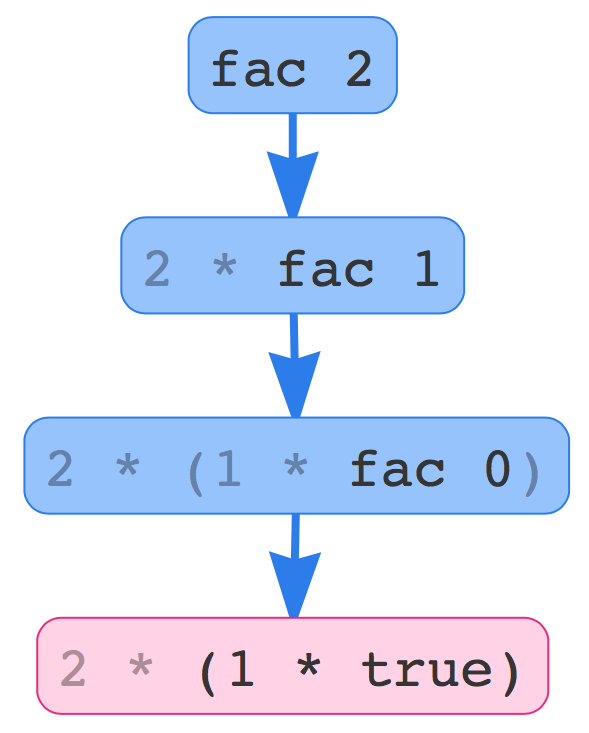
\includegraphics[height=1.5in]{fac-overview.png}
\end{minipage}
\begin{minipage}{.49\linewidth}
\centering
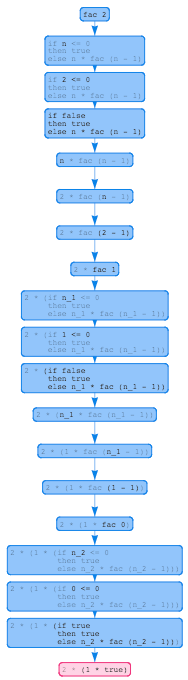
\includegraphics[height=3in]{fac-long.png}
\end{minipage}
\vspace{1em}
\caption{(top-left) An ill-typed \texttt{fac} function \hlOcaml{highlighting} the error location reported by \ocaml. (bottom-left) Dynamically witnessing the type error in \texttt{fac}, showing only function call-return pairs. (right) The same trace, fully expanded to show each small-step reduction in the computation.}
\label{fig:factorial}
\end{figure}

In this paper we propose a new approach that explains
static type errors by \emph{dynamically} witnessing
how an ill-typed program goes wrong.
%
We have developed \toolname, an interactive tool that uses
the source of the ill-typed function to automatically synthesize
the result on the bottom-left in Figure~\ref{fig:factorial}, which
shows how the recursive calls reduce to a configuration where
the program ``goes wrong'' --- \ie\ the @int@ value @1@ is to be
multiplied with the @bool@ value @true@.
We achieve this via three concrete contributions.

\paragraph{1. Finding Witnesses}
Our first contribution is an algorithm for searching for
\emph{witnesses} to type errors, \ie\ inputs that cause a
program to go wrong~(\S~\ref{sec:searching-witness}).
%
This problem is tricky when we cannot rely on
static type information, as we must avoid the
trap of \emph{spurious} inputs that cause
irrelevant problems that would be avoided
by picking values of a different, relevant type.
%
We solve this problem by developing a novel
operational semantics that combines evaluation
and type inference.
%
We execute the program with \emph{holes} --- values whose type is
unknown --- as the inputs.
%
A hole remains abstract until the evaluation
context tells us what type it must have, for
example the parameters to an addition operation
must both be integers.
%
Our semantics conservatively instantiates holes
with concrete values, dynamically inferring the
type of the input until the program goes wrong.
%
We prove that our procedure synthesizes \emph{general}
witnesses, which means, intuitively, that if a witness
is found for a given ill-typed function, then, \emph{for all}
(inhabited) input types, there exist values that can make
the function go wrong.

Given a witness to a type error, the novice may still be at a loss.
%
The standard \ocaml\ interpreter and debugging infrastructure expect
well-typed programs, so they cannot be used to investigate \emph{how}
the witness causes the program to crash.
%
More importantly, the execution itself may be quite long and may contain
details not relevant to the actual error.

\paragraph{2. Visualizing Witnesses}
Our second contribution is an interactive visualization of the
execution of purely functional \ocaml\ programs, well-typed or not~(\S~\ref{sec:interactive}).
%
We extend the semantics to also build a \emph{reduction graph}
which records all of the small-step reductions and the context
in which they occur.
%
The graph lets us visualize the sequence of
steps from the source witness to the stuck term. The user can
interactively expand the computation to expose intermediate steps
by selecting an expression and choosing a traversal strategy.
%
The strategies include many of the standard debugging moves, \eg\
stepping \emph{forward} or \emph{into} or \emph{over} calls, as well
stepping or jumping \emph{backward} to understand how a particular
value was created, while preserving a context of the intermediate
steps that allow the user to keep track of a term's provenance.

We introduce a notion of \emph{jump-compressed} traces to abstract away
the irrelevant details of a computation.
%
A jump-compressed trace includes only function
calls and returns, for example the trace in the bottom-left of
Figure~\ref{fig:factorial} is jump-compressed.
%
Jump-compressed traces are similar to stack traces, both show a
sequence of function calls that lead to a crash, but the jump-compressed
trace also shows the return values of successful calls, which can be
useful in understanding why a particular path was taken.

\paragraph{3. Evaluating Witnesses}
%
Of course, the problem of finding witnesses is
undecidable in general. In fact, due to the necessarily
conservative nature of static typing, there
may not even exist any witnesses for a given
ill-typed program.
%
Thus, our approach is a heuristic that is only useful
if it can find \emph{compact} witnesses for
\emph{real-world} programs.
%
Our third contribution is an extensive evaluation of our approach
on two different sets of ill-typed programs obtained by instrumenting
compilers used in beginner's classes~(\S~\ref{sec:evaluation}).
%
The first is the \uwbench\ data set~\cite{Lerner2007-dt}
comprising \uwsize\ ill-typed programs.
%
The second is a new \ucsdbench\ data set, comprising \ucsdsize\
ill-typed programs.
%
We show that for both data sets, our technique is able to generate
witnesses for nearly 90\% of the programs, in under a second in the
vast majority of cases.
%
Furthermore, we show that a simple interactive strategy yields
compact counterexample traces with at most 5 steps for 57\%
of the programs, and at most 10 steps for 81\% of the programs.

The ultimate purpose of an error report is to help the programmer
\emph{comprehend} and \emph{fix} problematic code.
%
Thus, our final contribution is a user study that compares \toolname's
dynamic witnesses against \ocaml's type errors along the dimension of
comprehensibility~(\S~\ref{sec:user-study}).
%
Our study finds that students given one of our witnesses are
consistently more likely to correctly explain and fix a type
error than those given the standard error message produced by
the \ocaml compiler.


%
% \subparagraph{Witness Utility}
%
% Even if we can find small witnesses for the majority of type errors, it
% may be that the witnesses do not actually help developers
% \emph{understand} the errors.
%
% In other words, perhaps the static error message is sufficient to
% diagnose and fix the error, or perhaps the witness simply does not add
% enough information to make a difference.
%
%
% Thus, our final contribution is a user study that compares the utility
% of our witnesses with that of the error messages provided by the \ocaml
% compiler~(\S~\ref{sec:user-study}).
%

\smallskip
All together, our results show that in the vast majority of cases, (novices') ill-typed
programs \emph{do} go wrong, and that the witnesses to these errors can be
helpful in understanding the source of the error. This, in turn, opens the
door to a novel dynamic way to explain, understand, and appreciate the
benefits of static typing.


%%% Local Variables:
%%% mode: latex
%%% TeX-master: "main"
%%% End:
